\documentclass{../TechDoc}

\usepackage{xcolor}
\usepackage{etoolbox}
\makeatletter
\patchcmd{\thebibliography}{%
	\chapter*{\bibname}\@mkboth{\MakeUppercase\bibname}{\MakeUppercase\bibname}}{%
	\section{References}}{}{}
\makeatother

\title{Анализ поведения временных систем с помощью динамических метрических графов.}
\author{Студент группы БПИ172}{А. А. Измайлов}
\academicTeacher{Доцент департамента программной инженерии
	факультета компьютерных наук}{Л. В. Дворянский}

\documentTitle{Пояснительная записка}
\documentCode{RU.17701729.04.01-01 ПЗ 81 01-1}

\addto\captionsrussian{\def\refname{Список используемых источников}}
\begin{document}
	\maketitle
	\tableofcontents
	
	\section{Введение}
	\subsection{Наименование программы}
	\subsubsection{Наименование на русском языке}
	Анализ поведения временных систем с помощью динамических метрических графов.
	\subsubsection{Наименование на английском языке}
	Behaviour analysis of real time systems via dynamic metric graphs.
	
	\subsection{Основание для разработки}
		Приказ декана факультета компьютерных наук И.В. Аржанцева "Об утверждении тем, руководителей курсовых работ студентов образовательной программы «Программная инженерия» факультета компьютерных наук" № 2.3-02/1112-04 от 11.12.2019.
	
	\section{Назначение разработки}
	\subsection{Назначение программы}
	\subsubsection{Функциональное назначение}
	Программа представляет из себя транслятор, который принимает на вход временную сеть Петри\cite{PetriNet}, а на выход выдает метрический граф\cite{MGraphs} или сообщение о том, что конвертация не возможна, а также наоборот. Программа не всегда может перевести сеть Петри в метрический граф, так как у этих моделей разная выразительность.
	\subsubsection{Эксплуатационное назначение}
	Данная программа может быть использована при исследовании свойств сетей Петри применительно к метрическим графам или наоборот. Такое может быть полезно, так как по отдельности эти две модели хорошо изучены, но методы исследования одной модели никто не применял к исследованию второй модели.
	
	\subsection{Краткая характеристика области применения}
	На данный момент временные сети Петри и метрические графы по отдельности хорошо изучены, но на самом деле между ними есть связь\cite{CorMgTapn}, что дает возможность применять методы анализа одной модели к другой, и наоборот. Так как данная сфера только начинает развиваться, на рынке нет автоматизированных решений для конвертации данных моделей друг к другу, зато уже давно есть программы для анализа временных сетей Петри, например UPPAAL\cite{uppaal}/TAPAAL\cite{tapaal},
	а также много результатов по изучению метрических графов. 
	
	
	Программа <<Анализ поведения временных систем с помощью динамических метрических графов>> позволяет проводить перевод сетей Петри в метрические графы и обртано, что должно помочь развивать данную сферу науки быстрее, так как не нужно будет в ручную переводить модели друг в друга для последующего анализа с помощью уже существующих решений.
	
	\section{Технические характеристики}
	\subsection{Постановка задачи на разработку программы}
	Программа должна:
	\begin{itemize}
		\item уметь считывать временную сеть Петри с внешнего хранилища;
		\item уметь считывать метрический граф с внешнего хранилища;
		\item конвертировать временную сеть Петри в метрический граф;
		\item предоставлять отчет о том, почему нельзя перевести сеть Петри в метрический граф;
		\item конвертировать метрический граф во временную сеть Петри;
	\end{itemize}
	
	\subsection {Описание алгоритма и функционирования программы}
	\subsubsection{Внутреннее представляени метрического графа}
		Метрический граф в программе представлен, как взвешенный ориентированный граф.
		Для обозночение бесконечного ребра одна из вершин помечается как бесконечность (со стороны графа это просто вершина), а длина ребра равняется бесконечность ( \textit{Double.POSITIVE\_INFINITY} в языке программирования Java).
		Метрические графы по определению неориентированные, но для однозначности понимания того, что происходит при столкновении двух точек на ребре, ребро представляется как пара из двух ориентированных ребер одной длинны.
		Каждое ребро хранит список точек на нем.
	\subsubsection{Конвертация метрического графа в временную Сеть Петри\cite{CorMgTapn}}
	\begin{enumerate}
		\item Для каждого ребра $e$ соединяющего вершины $a$ и $b$ создается место $e_{ab}$ и место $e_{ba}$.
		\item Для каждого ребра, у которого нет одного конца, т.е. пары ориентированных ребер из бесконечности (в нашей реализации у каждой бесконечности есть вершина, пусть это будет $a$) в $b$ и обратно в $a$.
		\begin{enumerate}
			\item Создается место $e_{ba}$ и соединение $t_{ba}$ со срочностью 0, ребро с нулевым интервалом из $e_{ba}$ в $t_{ba}$. (Рис. \ref{fig:mgtotapnlead})
			\item Для всех точек на ребре $ba$ создаются токены со временем 0 в месте $e_{ba}$
			\item Создается соединение $t_{ab}$ со срочностью 0.
			\item Для каждой точки $p_i$ на ребре $ab$
			\begin{enumerate}
				\item Создается место $e_{ab}^i$ c одним токеном
				\item Создается ребро из $e_{ab}^i$ в $t_{ab}$ с временным интервалом $[x(p_i), x(p_i)]$
			\end{enumerate}
			\item для каждого ребра $bc$ создается ребро из $t_{ab}$ в $e_{bc}$ 
		\end{enumerate}
		\item Для каждого созданного места ${e_{ab}}$ где $a$ не бесконечность.
		\begin{enumerate}
			\item Для каждой точки $p, x(p) = x_0$ на ориентированном ребре из $a$ в $b$ создается токен в месте $e_{ab}$ c значением таймера $x_0$.
			\item Далее для $e_{ab}$ рядом создается переход $t_{ab}$ со срочностью равной 0, если $b$ небесконечность
			\item Далее для $e_{ab}$ соединяестя ребром с временным интервалом равным $[l(e), l(e)]$ с $t_{ab}$.
			\item Для каждого ориентированного ребра выходящего из $b$ в вершину $c$ создается ребро из $t_{ab}$ в $e_{bc}$.
			\item создается еще одно соединение $\bar{t}_{ab}$. Также создается ребро двойной кратности с нулевым временным интервалом из $e_{ab}$ в $\bar{t}_{ab}$ и обратно одинарной кратности.
		\end{enumerate}
		\item Для получившейся сети запускается силовой алгоритм размещения Fruchterman and Reingold\cite{frlay}.
	\end{enumerate}

	По ходу алгоритма, новым объектам присваиваются идентификаторы:
		\begin{itemize}
			\item p\_\textit{id ребра} - имя места, полученного из соответствующего ребра
			\item t\_\textit{id ребра} - имя соединения, полученного из соответсвующего ребра
			\item ct\_\textit{id ребра} - имя соединения, для схлопования токенов, полученного из соответствующего ребра
		\end{itemize}

	Итоговая сложность $O(|E| \cdot max(cnt(e \in E)))$ для построения сети Петри без размещения, и $O(|V|^2 + |E|)$ для размещения, где $E$ - ребра, $V$ - вершины, $cnt$ - количество точек на ребре.
	\begin{figure}
		\centering
		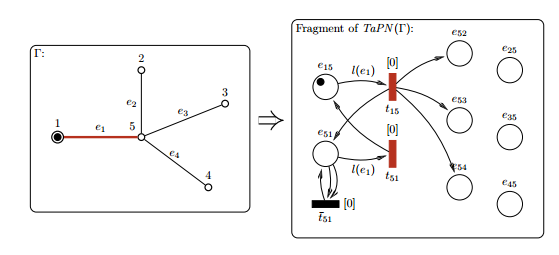
\includegraphics[width=0.5\linewidth]{mg_to_tapn_simple}
		\caption{Конвертация ребра $e_1$}
		\label{fig:mgtotapnsimple}
	\end{figure}
	\begin{figure}
		\centering
		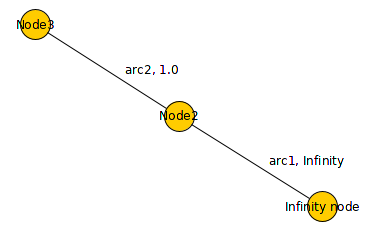
\includegraphics[width=0.3\linewidth]{mg_with_lead}
		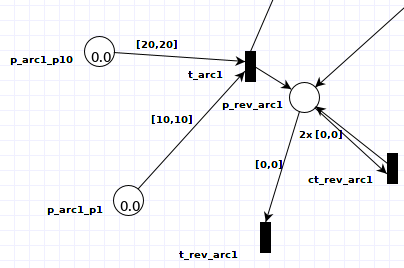
\includegraphics[width=0.3\linewidth]{mg_to_tapn_lead}
		\caption{Конвертация ребра $arc1$, которое идет из бесконечности, и содержит 2 точки, $rev\_arc1$ - обратное ребро в бесконечность. Для каждой точки получается свое место}
		\label{fig:mgtotapnlead}
	\end{figure}
	

	\subsubsection{Конвертация из временных сетей Петри в метрические графы\cite{CorMgTapn}}
		Из-за меньшей выразительности метрических графов, не все временные сети Петри могут быть переведены в метрические графы.
		Временная сеть петри может быть переведена, если:
		\begin{itemize}
			\item Все соединения имеют срочность 0
			\item Все временные интервалы имеют длинну 0, то есть содержат только одну точку.
		\end{itemize}
		
		Данные условия проверяются при первой встречи той или инной сущности в работе алгоритма.
		
		\begin{enumerate}
			\item Для каждого соединения $t_i$ создается вершина $v_i$ в графе.
			\item Для каждого соединения $t_i$, для всех исходящих из него ребер рассматривается место $p$, для всех исходящих ребер из $p$ расматривается соединение $t_j$.
			\begin{enumerate}
				\item Между соответсвующими вершинами $v_i$ и $v_j$ для $t_i$, $t_j$ проводится ребро с длиной равной временному интервалу, или очень маленькому числу, если интервал равен [0, 0].
				
				В данном шаге могут образоваться кратные ребра или ребра из вершины в неё же. Разрешается это так (Рис. \ref{fig:multiedgeres}):
				\begin{itemize}
					\item Для кратных ребер создается новая вершина, превращающая одно из ребер в два. Длина полученых ребер равна длине начального пополам.
					\item Для циклов с самим собой создается две дополнительные вершины, ребро делится на три ребра, длиной в три раза меньше
				\end{itemize}
				\item Для всех токенов из $p$ в начало полученного ребра из $v_i$ в $v_j$, то есть в вершину $v_i$, ставится точка.
			\end{enumerate}
			\item Для всех $p$, у которых есть только входный или только выходные ребра
			\begin{enumerate}
				\item для каждого соседнего соединения $t$ из соответсвуюшей вершины $v$ создается бесконечное ребро. 
				\item если у $p$ только исходящие ребра, то для каждого токена в $p$, для каждого исходящего ребра с концом в $t_i$, в бесконечное ребро из соответствующей вершины $v_i$ ставится точка в сторону к $v_i$, на расстоянии от $v_i$ равном временному интервалу на ребре из $p$ в $t_i$.  
			\end{enumerate}
		\end{enumerate}
	
	По ходу алгоритма, новым объектам присваиваются идентификаторы:
		\begin{itemize}
			\item a\_\textit{id соединения}\_\textit{id места}\_\textit{id соединения} - имя ребра, полученного из соотвествующих соединений и места
			\item rev\_\textit{id} - имя обратного ребра для ребра id
			\item l\_\textit{id начала}\_\textit{id конца} - имя ребра, соединеного с бесконечностью
			\item inf\_\textit{id начала}\_\textit{id конца} - имя для вершины бесконечности
			\item br\_\textit{id}\_part* - имя ребра для разлома цикла с самим собой или кратного ребра
			\item br\_n\_\textit{id} - имя вершины для разлома цикла с самим собой или кратного ребра
		\end{itemize}
	
	Итоговая сложность $O(|E| \cdot max(cnt(p \in P)))$ для построения метрического графа, где $E$ - множество ребер, $cnt$ - количество токенов в месте.
	
	\begin{figure}
		\centering
		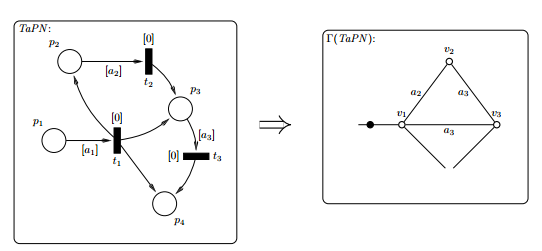
\includegraphics[width=0.5\linewidth]{tapn_to_mg}
		\caption{Конвертация сети Петри в Метрический граф}
		\label{fig:tapntomg}
	\end{figure}
	\begin{figure}
		\centering
		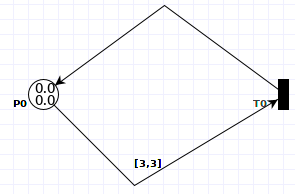
\includegraphics[width=0.3\linewidth]{multi_edge}
		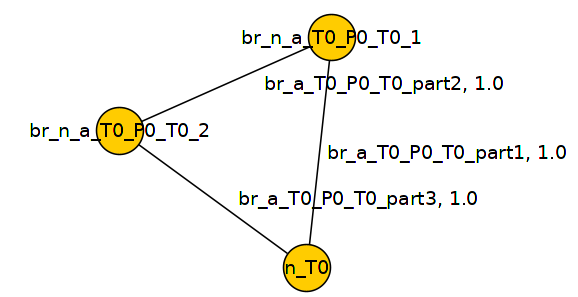
\includegraphics[width=0.3\linewidth]{multi_edge_res}
		\caption{Обход ситуации с циклом с самим собой}
		\label{fig:multiedgeres}
	\end{figure}
	
	\subsubsection{Сериализация метрических графов в формат JSON\cite{JSON}}
		Все ребра записываются в JSON, в виде объектов со всей дополнительной информацие, такой как \textbf{id} - идентификатор, \textbf{label} - метка, \textbf{comment} - комментарий. За ними записываются ребра, которые внутри себя содержат массив точек на этих ребрах и всю дополнительную информацию, как \textbf{id} - идентификатор, \textbf{label} - метка, \textbf{comment} - комментарий, \textbf{length} - длина.
		
		Сложность данного алгоритма $O(|V| + |E| \cdot max(cnt(e \in E)))$, где $V$ - множество вершин, $E$ - множество ребер, $cnt$ - количество точек на ребре.
		
	\subsubsection{Десериализация метрических графов из формата JSON}
		\begin{itemize}
			\item Входные данные валидируются по схеме\cite{jsonschema} см. Приложение 4
			\item С помощью SAX\cite{SAX} парсера данные достаются из файла, и складываются в промежуточные cписки ребер и вершин
			\item В объект \textit{builder}, который строит граф, кладутся сначала вершины, потом ребра.
			\item \textit{builder} строит граф, или сообщает об ошибке.
		\end{itemize}
	
		Сложность данного алгоритма $O(N + |V| + |E| \cdot max(cnt(e \in E)))$, где $N$ - размер входного файла, $V$ - множество вершин, $E$ - множество ребер, $cnt$ - количество точек на ребре.
		
	\subsubsection{Сериализация метрических графов в формат yEd GraphML\cite{yedgraphml}}
		Данная сериализация почти не отличается от JSON, кроме формата XML, и того, что для более красивого представления, обратные ребра нужно спрятать. Для этого, по ходу записи, ребра складываются в множество $s$. И при записи текущего ребра, если обратное ему содержится в $s$, то текущему ребру присваивается свойство \textbf{visible} = \textit{false}.
		
		Так же для присвоения вершина координат, используется силовой алгоритм размещения Fruchterman and Reingold, перед записью.
		
		Сложность записи $O(N + |V| + |E| \cdot max(cnt(e \in E)))$, сложность расположения $O(|V|^2 + |E|)$, где $N$ - размер входного файла, $V$ - множество вершин, $E$ - множество ребер, $cnt$ - количество точек на ребре.
		
	\subsubsection{Построение метрического графа}
		Для построения графа используется шаблон проектирования Builder\cite{builder}. Для внутреннего хранения используются структуры из JGraphT\cite{jgrapht}.
		
		Builder графа хранит внутри себя промежуточный граф, состоящий из вершин, и сырых ребер, которые тоже являются Builder, только для ребер.
		
		При любом изменении, Builder графа проверяет консистентность структуры графа:
		\begin{itemize}
			\item каждый объект: вершина, ребро, точка, имеют уникальный идентификатор
			\item нет кратных ребер
			\item нет ребер из бесконечности в бесконечность
			\item всегда есть обратное ребро
		\end{itemize}
		
		В Builder графа можно добавить:
		\begin{itemize}
			\item вершину
			\item ребро, между двумя добавленными вершинам, сразу с обратным ребром
			\item точку в уже добавленное ребро, это возможно благодаря тому, что хранится не ребро, а сырое ребро
		\end{itemize}
	
		После построения Builder порождает неизменяемый объект графа, который соотвествует всем свойствам метрического графа.
		
	\subsubsection{Механизм конвертации}
		С помощью шаблона проектирования Chain of Responsibility\cite{chain_resp}, конвертации можно выстроить в цепочку (или композицию, если говорить в функциональном стиле). 
		
		То есть можно сделать цепочки:
		\begin{itemize}
			\item файл $\rightarrow$ метрический граф $\rightarrow$ временная сеть Петри $\rightarrow$ файл
			\item файл $\rightarrow$ временная сеть Петри $\rightarrow$ метрический граф $\rightarrow$ файл
		\end{itemize}
		
		так как объекты реализуют интерфейс функции \textit{Function<TIn, TOut>}\cite{javafunction}.
		
	\subsubsection{Расширение TAPAAL}
		Чтобы расширить функциональность TAPAAL, и не получить циклических зависимостей был выбран механизм точек расширения\cite{extension}.
		
		В разных местах внутри кода TAPAAL объявляются точки расширения, которые являются проводником для дополнительной логики из вне. TAPAAL объявляет имя и интерфейс для общения с расширениями, это и называется точкой расширения. 
		
		В другом месте, вне TAPAAL, можно объявить расширения, объявив тем самым новую логику, не изменяя код TAPAAL и не добавляя зависимостей в модуль TAPAAL.
		
		В данной программе, реализовано 3 расширения, которые добавляют новый элементы для вызова конвертаций в меню. 
		
	\subsubsection{Обоснование выбора алгоритмов решения задания}
		\begin{itemize}
			\item Алгоритмы конвертации являются на данный момент единственными, поэтому они были выбраны.
			\item SAX десериализация была выбрана, так как она за один проход дает возможность считать данные, без хранения лишних данных.
			\item Шаблон Builder для построения графа, позволяет инкапсулировать логику валидации, и сделать создание графа атомарным действием, то есть либо графа не сущесивуеи, либо он есть сразу со всеми содержимым.
		\end{itemize}
	
	\subsubsection{Возможные взаимодействия программы с другими программами}
		Данная программа может быть вызвана через CLI из другой прогрыммы, так же другие программы могут объявлять свои точки расширения для TAPAAL, добавляя свою логику.
		Созданные программой файлы .tapn можно открыть в TAPAAL, .graphml в yEd Graph Editor и в других программах, поддерживающих данный формат.
		
	\subsection{Описание и обоснование выбора метода организации входных и
выходных данных}
	\subsubsection{Описание метода организации входных и выходных данных}
		Входные/выходные данные для временных сетей Петри ораганизованы в XML\cite{XMl} формате TAPN, который является подмножеством PNML\cite{PNML}, стандартный формат данных в программе для анализа временных сетей Петри TAPAAL.
		
		Входные/Выходные данные представляются ввиде JSON, со своей схемой для валидации.
		
		Выходные данные для метрических графов так же могут быть в формате yEd GraphML, который является расширением GraphML\cite{graphml}, cтандартным форматом для yEd Graph Edito\cite{yededitor}.
		
	\subsubsection{Обоснования выбора метода организации входных и выходных данных}
		Формат TAPN выбран для совместимости с TAPAAL. Формат yEd GraphML выбран для использования программы yEd Graph Editor для визуализации полученных графов. 
		
		Формат JSON выбран потому что,
		 \begin{enumerate}
		 	\item JSON позволяет быстро считатывать и записывать данные, так как хранит только то, что нужно
		 	\item В данное время есть денденция выносить вычисления в облачные сервисы, где основным стандартом формата данных является JSON, нельзя исключать такой вариант развития данной программы.
		 \end{enumerate}
	 
	 \subsection{Описание и обоснование выбора состава технических и программных средств}
	 \subsubsection{Состав технических и программных средств}
	 
	 Для работы программы необходим следующий состав технических средств\cite{javareq}:
	 \begin{itemize}
	 	\item Процессор архитектуры AMD или Intel с частотой не менее 2 266 МГц;
	 	\item Не менее 512 МБ ОЗУ;
	 	\item Не менее 200МБ на жестком диске;
	 	\item Клавиатура;
	 \end{itemize}
	 
	 Для работы программы необходим следующий состав программных средств\cite{javareq}
	 \begin{itemize}
	 	\item Одна из ниже перечисленных операционных систем:
	 	\begin{itemize}
	 		\item Windows 10
	 		\item Windows 8.x (настольная версия)
	 		\item Windows 7 с пакетом обновления 1 (SP1)
	 		\item Windows Vista SP2
	 		\item Windows Server 2008 R2 с пакетом обновления 1 (SP1) (64-разрядная версия)
	 		\item Windows Server 2012 и 2012 R2 (64-разрядная версия)
	 		\item Mac OS X 10.8.3+, 10.9+
	 		\item Oracle Linux 5.5+1
	 		\item Oracle Linux 6.x (32-разрядная версия), 6.x (64-разрядная версия)2
	 		\item Oracle Linux 7.x (64-разрядная версия)2
	 		\item Red Hat Enterprise Linux 5.5+1, 6.x (32-разрядная версия), 6.x (64-разрядная версия)2
	 		\item Red Hat Enterprise Linux 7.x (64-разрядная версия)2
	 		\item Suse Linux Enterprise Server 10 SP2+, 11.x
	 		\item Suse Linux Enterprise Server 12.x (64-разрядная версия)2
	 		\item Ubuntu Linux 12.04 LTS, 13.x, 14.x, 15.x, 16.x, 18.x
	 	\end{itemize}
	 	\item Установленная Java SE Runtime Environment 11 или выше
	 \end{itemize}
	 
	 \subsubsection{Обоснование выбора технических и программных средств}
	 Программа реализована на языке Java версии 11\cite{Java11}, с использованием библиотек, полностью написанных на Java. В программе используется много особенностей добавленных в Java 11, поэтому версия ниже не подойдёт.
	 
	 \section{Ожидаемые технико-экономические показатели}
	 \subsection{Предполагаемая потребность}
		 Данная программа может быть полезна при изучении совместных свойств метрических графов и временных сетей Петри. 
	 
	 \subsection{Экономические преимущества разработки по сравнению с отечественными и зарубежными аналогами}
		 Данная программа является первой реализацией конвертаций метрических графов в сети Петри и обратно, так как эта сфера только начинает развиваться.
		 
	\newpage
	\bibliographystyle{utf8gost705u}  %% стилевой файл для оформления по ГОСТу
	\bibliography{../biblio}     %% имя библиографической базы (bib-файла)
	\addtocounter{section}{2}
	\addcontentsline{toc}{section}{Список используемых источников}
	
	\section*{Приложение 1. Диаграмма модулей}
	\addcontentsline{toc}{section}{Приложение 1. Диаграмма модулей}	
	\begin{figure}[h!]
		\centering
		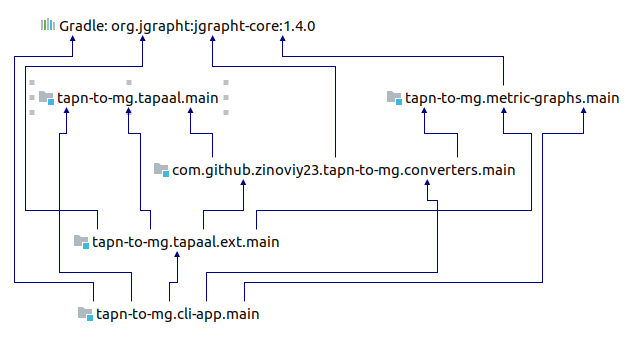
\includegraphics[width=0.9\linewidth]{modules_diagram}
		\caption{Диаграмма модулей}
		\label{fig:modulesdiagram}
	\end{figure}
	
	
	\section*{Приложение 2. Диаграмма классов}
	\addcontentsline{toc}{section}{Приложение 1. Диаграмма классов}
	\begin{figure}[h!]
		\centering
		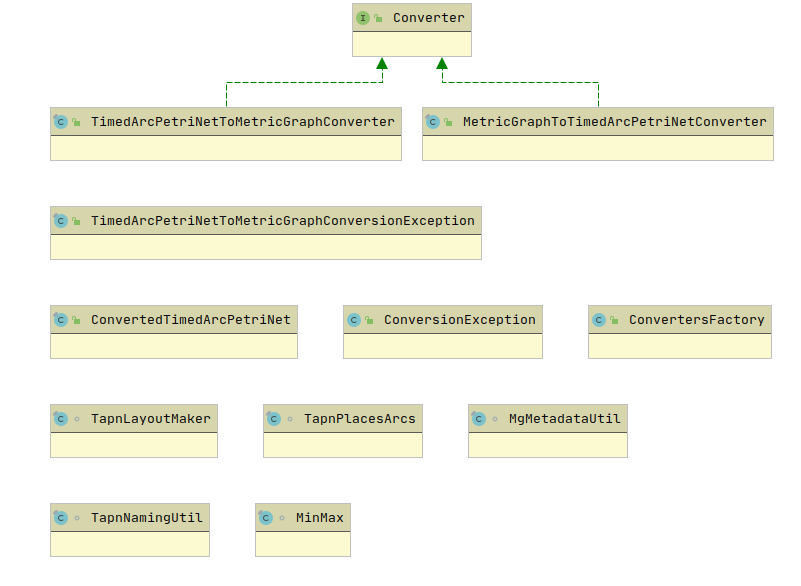
\includegraphics[width=0.9\linewidth]{converters_classes}
		\caption{Диаграмма классов модуля converters}
		\label{fig:convertersclasses}
	\end{figure}
	
	\begin{figure}[h!]
		\centering
		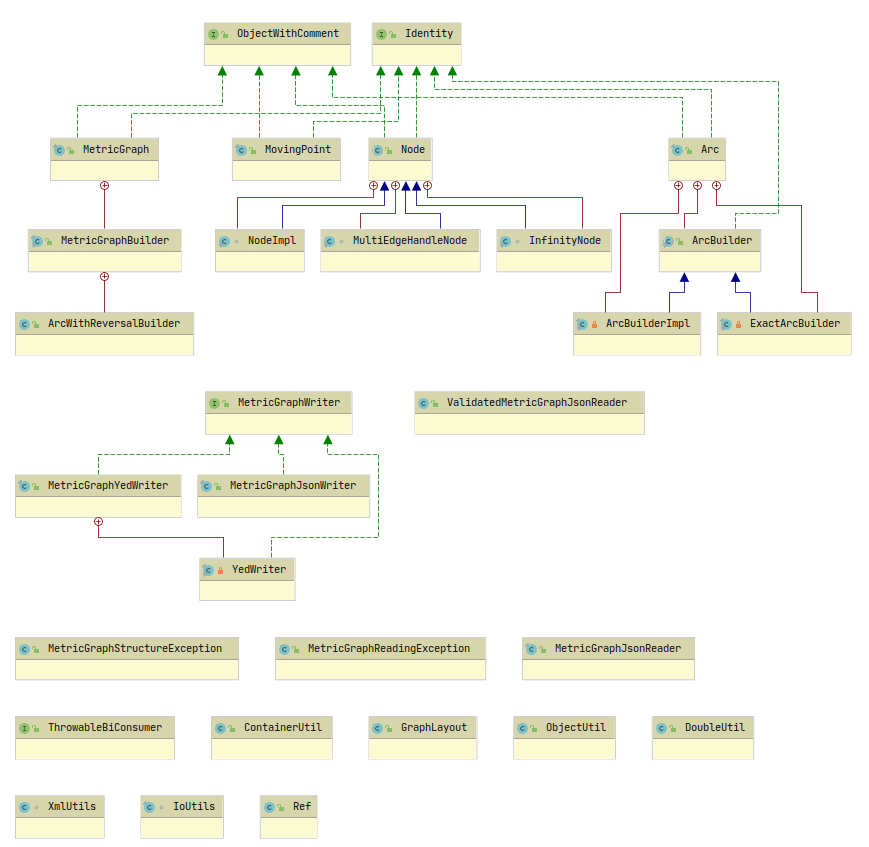
\includegraphics[width=0.9\linewidth]{mg_classes}
		\caption{Диаграмма классов модуля metric-graphs}
		\label{fig:mgclasses}
	\end{figure}
	
	\begin{figure}[h!]
		\centering
		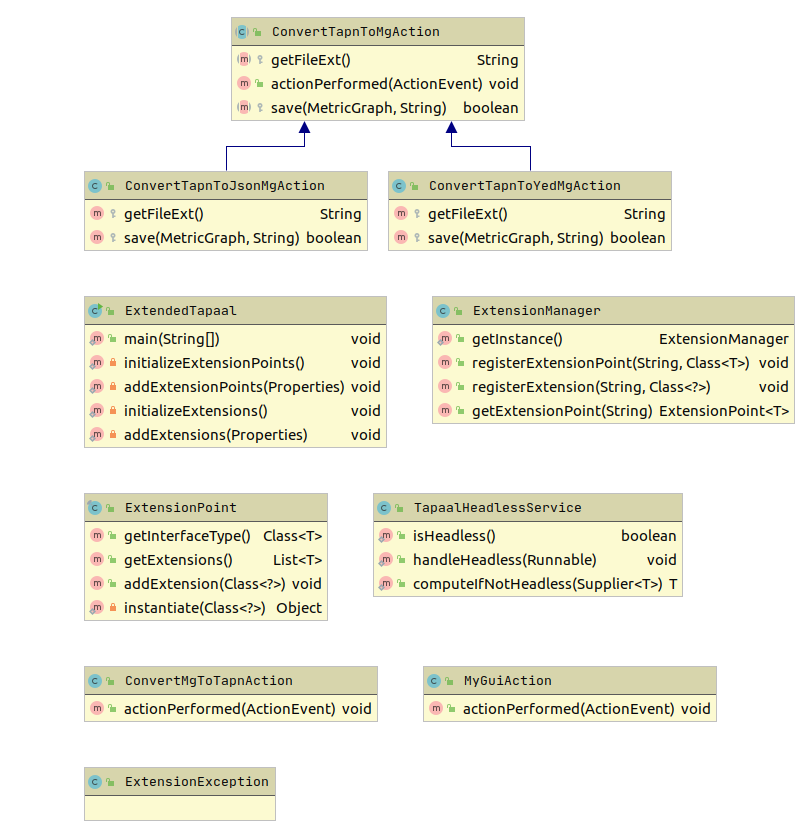
\includegraphics[width=0.9\linewidth]{ext_classes}
		\caption{Диаграмма классов модуля tapaal.ext}
		\label{fig:extclasses}
	\end{figure}
	
	\section*{Приложение 3. JSON схема для метрических графов}
	\addcontentsline{toc}{section}{Приложение 3. JSON схема для метрических графов}
	\lstinputlisting{json-graph-schema.json}
							
	\section*{Приложение 4. Описание и функциональное назначение
классов}
	\addcontentsline{toc}{section}{Приложение 4. Описание и функциональное назначение классов}	
	\begin{flushright}
		Таблица 4.1
	\end{flushright}
	\begin{tabular}{|l|m{17em}|}
		\hline
		\textbf{Класс} & \textbf{Назначение} \\
		\hline
		TapnToMg & Главный класс CLI\\
		\hline
		ConvertedTimedArcPetriNet & Результат конвертации из метрического графа в сеть Петри\\
		\hline
		MetricGraphToTimedArcPetriNetConverter & Конвертер из метрического графа в сеть Петри\\
		\hline
		MinMax & Класс для агрегации из коллекции минимума и максимума\\
		\hline
		TapnLayoutMaker & Класс для расположения вершин сети Петри\\
		\hline
		TapnNamingUtil & Класс для именования объектов в сети Петри\\
		\hline
		MgMetadataUtil & Класс для именования объектов в метрическом графе\\
		\hline
		TapnPlacesArcs & Класс для обращения к ребрам инцидентным местам в сети Петри\\
		\hline
		TimedArcPetriNetToMetricGraphConversionException & Исключение при конвертации из сети Петри в метрический граф\\
		\hline
		TimedArcPetriNetToMetricGraphConverter & Конвертер из сетей Петри в метрические графы\\
		\hline
		ConversionException & Исключение при конвертации\\
		\hline
		Converter & Общий класс для конвертаций\\
		\hline
		ConvertersFactory & Фабрика конвертеров \\
		\hline
		ObjectWithComment & Объект с комментарием\\
		\hline
		MetricGraphYedWriter & Класс для записи в формате yEd\\
		\hline
		XmlUtils & Методы для работы с XML\\
		\hline
		MetricGraphJsonReader & Класс для считывания с JSON \\
		\hline
		MetricGraphJsonWriter & Класс для записи в JSON\\
		\hline
		MetricGraphReadingException & Исключение при считывание\\
		\hline
		MetricGraphWriter & Общий класс для записи графов\\
		\hline
		ValidatedMetricGraphJsonReader & Класс для считывания с валидацией\\
		\hline
		ContainerUtil & Методы для работы с коллекциями\\
		\hline
		DoubleUtil & Методы для работы с числами\\
		\hline
		GraphLayout & Класс для расположения графов\\
		\hline
		ObjectUtil & Методы для работы с объектами\\
		\hline
		Ref & Ссылка на значение \\
		\hline
		ThrowableBiConsumer & Функциональный интерфейс для принятия 2х значений\\
		\hline
		Arc & Класс ребро\\
		\hline
		MetricGraph & Класс граф\\
		\hline
		MetricGraphStructureException & Ошибка в структуре графа\\
		\hline
		MetricGraphBuilder & Класс для построения графа\\
		\hline
		ArcBuilder & Общий класс для построения ребра\\
		\hline
		ArcBuilderImpl & Реализация класс для построения ребра\\
		\hline
		ExactArcBuilder & Реализация, которая возврощает заданное ребро\\
		\hline
	\end{tabular}
	
	\begin{flushright}
		Продолжение таблицы 4.1
	\end{flushright}
	\begin{tabular}{|l|m{20em}|}
		\hline
		\textbf{Класс} & \textbf{Назначение} \\
		\hline
		YedWriter & Класс для записи в yEd XML\\
		\hline
		MovingPoint & Класс точка \\
		\hline
		Node & Класс вершина\\
		\hline
		ExtensionException & Ошибка при расширении\\
		\hline
		ExtensionManager & Класс для управления расширениями \\
		\hline
		ExtensionPoint & Представление точки расширений \\
		\hline
		TapaalHeadlessService & Класс для контроля headless режима\\
		\hline
		ConvertMgToTapnAction & Класс для действия конвертации в сеть Петри\\
		\hline
		ConvertTapnToJsonMgAction & Класс для действия конвертации в JSON\\
		\hline
		ConvertTapnToMgAction &  Общий класс для действий конвертации\\
		\hline
		ConvertTapnToYedMgAction & Класс для действия конвертации в yEd \\
		\hline
		ExtendedTapaal & Главный класс расширенного TAPAAL \\
		\hline
		Identity & объект с id \\
		\hline
	\end{tabular}
	
	\section*{Приложение 5. Описание и функциональное назначение полей и методов}
	\addcontentsline{toc}{section}{Приложение 5. Описание и функциональное назначение полей и методов}	
	\begin{flushright}
		Таблица 5.1
	\end{flushright}
	Класс TapnToMg
	
	\begin{tabular}{|p{5cm}|p{5cm}|p{5cm}|}
		\hline
		\textbf{Имя} & \textbf{Модификатор доступа} & \textbf{Назначение} \\
		\hline
		main & public & главный метод \\
		\hline
	\end{tabular}
	\begin{flushright}
		Таблица 5.2
	\end{flushright}
	Класс ConvertedTimedArcPetriNet
	
	\begin{tabular}{|p{5cm}|p{5cm}|p{5cm}|}
		\hline
		\textbf{Имя} & \textbf{Модификатор доступа} & \textbf{Назначение} \\
		\hline
		getNetwork & public & возвращает временную сеть Петри\\
		\hline
		getTemplate & public & возвращает шаблон\\
		\hline
	\end{tabular}
	\begin{flushright}
		Таблица 5.3
	\end{flushright}
	Класс MetricGraphToTimedArcPetriNetConverter
	
	\begin{tabular}{|p{5cm}|p{5cm}|p{5cm}|}
		\hline
		\textbf{Имя} & \textbf{Модификатор доступа} & \textbf{Назначение} \\
		\hline
		addPlacesForEachArc & private & добавляет места для каждого ребра\\
		\hline
		processArc & private & обрабатывает ребро\\
		\hline
		addArcForNeighbours & private & добавляет ребра для соседей\\
		\hline
		handleInfinity & private & обрабатывает бесконечные вершины\\
		\hline
		
	\end{tabular}
	\begin{flushright}
		Таблица 5.4
	\end{flushright}
	Класс MinMax
	
	\begin{tabular}{|p{5cm}|p{5cm}|p{5cm}|}
		\hline
		\textbf{Имя} & \textbf{Модификатор доступа} & \textbf{Назначение} \\
		\hline
		reduce & package-private & изменяет мин/макс на входящее число\\
		\hline
		combine & package-private & комбинирует 2 объетка\\
		\hline
		avg & package-private & среднее из мин макс\\
		\hline
	\end{tabular}
	\begin{flushright}
		Таблица 5.5
	\end{flushright}
	Класс TapnLayoutMaker
	
	\begin{tabular}{|p{5cm}|p{5cm}|p{5cm}|}
		\hline
		\textbf{Имя} & \textbf{Модификатор доступа} & \textbf{Назначение} \\
		\hline
		getTextFromId & private & возвращает описание по id\\
		\hline
		createDataLayer & public & создает расположение графа\\
		\hline
		createNote & private & создает описание сети Петри\\
		\hline
		createPetriNetObject& public & по абстрактному объекту в графе расположения создает элемент сети Петри\\
		
		\hline
	\end{tabular}
	\begin{flushright}
		Таблица 5.6
	\end{flushright}
	Класс TapnNamingUtil
	
	\begin{tabular}{|p{5cm}|p{5cm}|p{5cm}|}
		\hline
		\textbf{Имя} & \textbf{Модификатор доступа} & \textbf{Назначение} \\
		\hline
		getTapnName& package-private & имя сети Петри \\
		\hline
		nameForPlace& package-private & имя для места\\
		\hline
		nameForTransition& package-private & имя для соединения\\
		\hline
		nameForCollapsingTransition& package-private & имя для схлопывающего места\\
		\hline
		nameForInfinitePlace& package-private & имя для бесконечного места\\
		
		\hline
	\end{tabular}
	\begin{flushright}
		Таблица 5.7
	\end{flushright}
	Класс MgMetadataUtil
	
	\begin{tabular}{|p{5cm}|p{5cm}|p{5cm}|}
		\hline
		\textbf{Имя} & \textbf{Модификатор доступа} & \textbf{Назначение} \\
		\hline
		getNodeName& private-package & имя для вершины\\
		\hline
		getNodeComment& private-package& коммент для вершины\\
		\hline
		getArcName&private-package & имя для ребра\\
		\hline
		getNameForReversal&private-package & имя для обратного ребра\\
		\hline
		getTokenName&private-package & имя для точек по токену\\
		\hline
		getLeadName&private-package & имя для ребра с одной вершиной\\
		\hline
		getInfName& private-package& имя для бесконечной вершины\\
		\hline
		getGraphName& private-package& имя графа\\
		\hline
		getMultiedgeHandlerNodeName& private-package& имя для вершины ломающей кратное ребро\\
		\hline
		getMultiedgeHandlerArcsNames&private-package & имя для ребер ломающих кратное ребро\\
		\hline
		getSelfLoopHandleArcsNames& private-package& имя для ребер ломающих цикл с самим собой\\
		\hline
		getComment&private-package & комментарий к графу \\
		
		\hline
	\end{tabular}
	\begin{flushright}
		Таблица 5.8
	\end{flushright}
	Класс TapnPlacesArcs
	
	\begin{tabular}{|p{5cm}|p{5cm}|p{5cm}|}
		\hline
		\textbf{Имя} & \textbf{Модификатор доступа} & \textbf{Назначение} \\
		\hline
		getOutputArcs & public & возвращает выходные ребра для места\\
		\hline
		getInputArcs& public & возвращает входные ребра для места\\
		\hline
		assertInputArc& private & провряет выходное ребро\\
		
		\hline
	\end{tabular}
	
	\begin{flushright}
		Таблица 5.9
	\end{flushright}
	Класс TimedArcPetriNetToMetricGraphConverter
	
	\begin{tabular}{|p{5cm}|p{5cm}|p{5cm}|}
		\hline
		\textbf{Имя} & \textbf{Модификатор доступа} & \textbf{Назначение} \\
		\hline
		addNodes& private & добавляет вершины\\
		\hline
		addEdges& private& добавляет ребра\\
		\hline
		addEdge& private& добавляет ребро\\
		\hline
		fixSelfLoop& private& возвращает ребра для починки цикла с самим собой\\
		\hline
		fixLength& private& возвращает длину ребра, всегда больше 0\\
		\hline
		getPointsFromPlace& private& точки из токенов в текущем месте\\
		\hline
		addLeads&private& добавляет ребра с одной вершиной\\
		\hline
		getPointsFromInputArc& private& добавляет точки из входного ребра \\
		\hline
		assertTransition&private & проверяет соединения\\
		
		\hline
	\end{tabular}

	\begin{flushright}
		Таблица 5.10
	\end{flushright}
	Класс Converter
	
	\begin{tabular}{|p{5cm}|p{5cm}|p{5cm}|}
		\hline
		\textbf{Имя} & \textbf{Модификатор доступа} & \textbf{Назначение} \\
		\hline
		convert& public & конвертирует A в B\\
		
		\hline
	\end{tabular}
	\begin{flushright}
		Таблица 5.11
	\end{flushright}
	Класс ConvertersFactory
	
	\begin{tabular}{|p{9cm}|p{2cm}|p{5cm}|}
		\hline
		\textbf{Имя} & \textbf{Модификатор доступа} & \textbf{Назначение} \\
		\hline
		createMetricGraphToTimedArcPetriNetConverter& public & создает конвертер из файла с графом в файл с сетью Петри \\
		\hline
		createFileToMetricGraphConverter&public & создает конвертер из файла в метрический граф \\
		\hline
		createTimedArcPetriNetToFileConverter& public& создает конвертер из сети Петри в файл\\
		\hline
		createFileToTimedArcPetriNetConverter& public& создает конвертер из файла в сеть петри\\
		
		\hline
	\end{tabular}

	\begin{flushright}
		Таблица 5.12
	\end{flushright}
	Класс Identity
	
	\begin{tabular}{|p{5cm}|p{5cm}|p{5cm}|}
		\hline
		\textbf{Имя} & \textbf{Модификатор доступа} & \textbf{Назначение} \\
		\hline
		getId& public& возвращает id\\
		
		\hline
	\end{tabular}

	\begin{flushright}
		Таблица 5.13
	\end{flushright}
	Класс ObjectWithComment
	
	\begin{tabular}{|p{5cm}|p{5cm}|p{5cm}|}
		\hline
		\textbf{Имя} & \textbf{Модификатор доступа} & \textbf{Назначение} \\
		\hline
		getComment &public & возвращает комментарий \\
		
		\hline
	\end{tabular}
	\begin{flushright}
		Таблица 5.14
	\end{flushright}
	Класс MetricGraphYedWriter
	
	\begin{tabular}{|p{5cm}|p{5cm}|p{5cm}|}
		\hline
		\textbf{Имя} & \textbf{Модификатор доступа} & \textbf{Назначение} \\
		\hline
		addIndents& private & добавляет отступы к XML\\
		
		\hline
	\end{tabular}
	
	\begin{flushright}
		Таблица 5.15
	\end{flushright}
	Класс MetricGraphJsonReader
	
	\begin{tabular}{|p{5cm}|p{5cm}|p{5cm}|}
		\hline
		\textbf{Имя} & \textbf{Модификатор доступа} & \textbf{Назначение} \\
		\hline& & \\
		\hline
		read & public & считывает граф \\
		\hline
		internalRead& private & считывает граф\\
		\hline
		readGraph&private & считывает и собирает граф\\
		\hline
		addArcAndReversal&private & добавляет ребро и обратное к нему\\
		\hline
		readEdges&private & считывает ребра\\
		\hline
		readEdge&private & считывает ребро\\
		\hline
		readArcMetadata&private & считвыает метаинформацию ребра\\
		\hline
		readPoints& private& считывает точки ребра\\
		\hline
		readPoint&private & считывает точку\\
		\hline
		readNodes&private & считывает вершины\\
		\hline
		readNode& private& считывает вершину\\
		\hline
		fetchMetadata& private& достае метаинформацию\\
		\hline
		lastLocation& public & последнее положение в файле до ошибки\\
		
		\hline
	\end{tabular}
	\begin{flushright}
		Таблица 5.16
	\end{flushright}
	Класс MetricGraphJsonWriter
	
	\begin{tabular}{|p{5cm}|p{5cm}|p{5cm}|}
		\hline
		\textbf{Имя} & \textbf{Модификатор доступа} & \textbf{Назначение} \\
		\hline
		internalWrite& private & записывает граф\\
		\hline
		writeGraphInfo& private& записывает дополнительную информацию о графе\\
		\hline
		writeNodes&private & записывает вершины\\
		\hline
		writeEdges& private& записывает ребра\\
		\hline
		writeArcMetadata&private & записывает метаинформацию ребра\\
		\hline
		writeComment&private & записывает комментарий\\
		
		\hline
	\end{tabular}
	\begin{flushright}
		Таблица 5.17
	\end{flushright}
	Класс MetricGraphWriter
	
	\begin{tabular}{|p{5cm}|p{5cm}|p{5cm}|}
		\hline
		\textbf{Имя} & \textbf{Модификатор доступа} & \textbf{Назначение} \\
		\hline
		write& public& записывает граф\\
		
		\hline
	\end{tabular}
	\begin{flushright}
		Таблица 5.18
	\end{flushright}
	Класс ValidatedMetricGraphJsonReader
	
	\begin{tabular}{|p{5cm}|p{5cm}|p{5cm}|}
		\hline
		\textbf{Имя} & \textbf{Модификатор доступа} & \textbf{Назначение} \\
		\hline
		validate& private & валидирует входной поток по схеме\\
		\hline
		getReader& public & возвращает внутренний считыватель\\
		
		\hline
	\end{tabular}
	\begin{flushright}
		Таблица 5.19
	\end{flushright}
	Класс ContainerUtil
	
	\begin{tabular}{|p{5cm}|p{5cm}|p{5cm}|}
		\hline
		\textbf{Имя} & \textbf{Модификатор доступа} & \textbf{Назначение} \\
		\hline
		first& public & первый элемент в коллекции \\
		\hline
		second&public & второй элемент в коллекции\\
		\hline
		getFromTable&public & достает элемент из таблицы\\
		\hline
		iterate&public & конвертирует Stream в Iterable\\
		
		\hline
	\end{tabular}
	\begin{flushright}
		Таблица 5.20
	\end{flushright}
	Класс DoubleUtil
	
	\begin{tabular}{|p{5cm}|p{5cm}|p{5cm}|}
		\hline
		\textbf{Имя} & \textbf{Модификатор доступа} & \textbf{Назначение} \\
		\hline
		equals& public& сравнивает два вещественных числа с учетом бесконечности и погрешности \\
		
		\hline
	\end{tabular}
	\begin{flushright}
		Таблица 5.21
	\end{flushright}
	Класс GraphLayout
	
	\begin{tabular}{|p{5cm}|p{5cm}|p{5cm}|}
		\hline
		\textbf{Имя} & \textbf{Модификатор доступа} & \textbf{Назначение} \\
		\hline
		createLayout& public & создает расположения графа\\
		\hline
		calcSize& private & считает размер области, в которой нужно разместить граф\\
		
		\hline
	\end{tabular}
	\begin{flushright}
		Таблица 5.22
	\end{flushright}
	Класс ObjectUtil
	
	\begin{tabular}{|p{5cm}|p{5cm}|p{5cm}|}
		\hline
		\textbf{Имя} & \textbf{Модификатор доступа} & \textbf{Назначение} \\
		\hline
		doIfNotNull& public& делает переданное действие, если первый аргумент не null\\
		
		\hline
	\end{tabular}
	\begin{flushright}
		Таблица 5.23
	\end{flushright}
	Класс Ref
	
	\begin{tabular}{|p{5cm}|p{5cm}|p{5cm}|}
		\hline
		\textbf{Имя} & \textbf{Модификатор доступа} & \textbf{Назначение} \\
		\hline
		getData& public & возвращает содержимое\\
		\hline
		setData&public & обновляет содержимое\\
		\hline
		update&public & обновляет содержимое с помощью переданной функции\\
		
		\hline
	\end{tabular}
	\begin{flushright}
		Таблица 5.24
	\end{flushright}
	Класс ThrowableBiConsumer
	
	\begin{tabular}{|p{5cm}|p{5cm}|p{5cm}|}
		\hline
		\textbf{Имя} & \textbf{Модификатор доступа} & \textbf{Назначение} \\
		\hline
		consume& public& принимает два аргумента и обрабатывает 2 аргумента\\
		
		\hline
	\end{tabular}
	\begin{flushright}
		Таблица 5.25
	\end{flushright}
	Класс Arc
	
	\begin{tabular}{|p{5cm}|p{5cm}|p{5cm}|}
		\hline
		\textbf{Имя} & \textbf{Модификатор доступа} & \textbf{Назначение} \\
		\hline
		createBuilder& public & создает Builder ребра\\
		\hline
		verifyLength& private & проверяет длину ребра\\
		\hline
		checkPointsOnArc& package-private& проверяет что точки находятся на ребре\\
		\hline
		getLabel&public & возвращает метку\\
		\hline
		getSource&public & возвращает начальную вершину\\
		\hline
		getTarget&public & возвращает конечную вершину\\
		\hline
		getLength& public& возвращает длину\\
		\hline
		getPoints&public & возвращает точки\\
		\hline
		isDistanceToTarget&public & возвращает, считается ли расстояние с конца ребра\\
		\hline
		toBuilder&package-private & преварщает ребро в Builder ребра\\
		
		\hline
	\end{tabular}
	\begin{flushright}
		Таблица 5.26
	\end{flushright}
	Класс MetricGraph
	
	\begin{tabular}{|p{5cm}|p{5cm}|p{5cm}|}
		\hline
		\textbf{Имя} & \textbf{Модификатор доступа} & \textbf{Назначение} \\
		\hline
		createBuilder& public & создает Builder графа\\
		\hline
		getGraph&public & возвращает структуру графа\\
		\hline
		getLabel&public & возвращает метку\\
		\hline
		getReversal&public & обратное ребро\\
		\hline
		getNode& public& возвращает вершину по id\\
		\hline
		getArc& public& возвращает ребро по id\\
		
		\hline
	\end{tabular}
	\begin{flushright}
		Таблица 5.27
	\end{flushright}
	Класс MetricGraphBuilder
	
	\begin{tabular}{|p{5cm}|p{5cm}|p{5cm}|}
		\hline
		\textbf{Имя} & \textbf{Модификатор доступа} & \textbf{Назначение} \\
		\hline
		buildGraph& public & строит граф\\
		\hline
		addNode& public& добавляет вершину\\
		\hline
		addArc& public& добавляет ребро\\
		\hline
		setLabel& public& добавляет метку\\
		\hline
		setComment& public& присваивает комментарий\\
		\hline
		setId& public& присваивает идентификатор\\
		\hline
		addPoints&public & добавляет точки\\
		\hline
		containsEdge& public& проверяет есть ли ребро\\
		\hline
		verifyPoints& private& проверяет точки\\
		\hline
		addPoints& private& добавляе идентификаторы точек\\
		\hline
		verifyId& private& проверят идентификатор\\
		\hline
		addId& private& добавляет идентификатор\\
		\hline
		failAlreadyExists& private& кидает исключение, если объект уже есть\\
		\hline
	\end{tabular}
	\begin{flushright}
		Таблица 5.28
	\end{flushright}
	Класс ArcBuilder
	
	\begin{tabular}{|p{5cm}|p{5cm}|p{5cm}|}
		\hline
		\textbf{Имя} & \textbf{Модификатор доступа} & \textbf{Назначение} \\
		\hline
		setSource&public & присваивает начало ребра\\
		\hline
		getSource&public & возвращает начало ребра\\
		\hline
		setTarget&public & присваивает конец ребра\\
		\hline
		getTarget&public & возвращает конец ребра\\
		\hline
		setLength&public & присваивает длину\\
		\hline
		getLength&public & возвращает длину\\
		\hline
		addPoint&public & добавляет точку\\
		\hline
		createArc&public & создает ребро\\
		\hline
		setId& public& присваивает идентификатор\\
		\hline
		getPoints&public & возвращает точки\\
		\hline
		setPoints&public & присваивает точки\\
		\hline
		getLabel&public & возвращает метку\\
		\hline
		setLabel&public & присваивает точку\\
		\hline
		getComment&public & возвращает коммент\\
		\hline
		setComment&public & присваивает коммент\\
		\hline
		copy&public & копирует объект\\
		\hline
		makeString& protected& создает строку для toString\\
		
		\hline
	\end{tabular}
	\begin{flushright}
		Таблица 5.29
	\end{flushright}
	Класс ArcBuilderImpl
	
	\begin{tabular}{|p{5cm}|p{5cm}|p{5cm}|}
		\hline
		\textbf{Имя} & \textbf{Модификатор доступа} & \textbf{Назначение} \\
		\hline
		verifyPointId& private & проверяет идентификатор точки \\
		
		\hline
	\end{tabular}
	\begin{flushright}
		Таблица 5.30
	\end{flushright}
	Класс YedWriter
	
	\begin{tabular}{|p{5cm}|p{5cm}|p{5cm}|}
		\hline
		\textbf{Имя} & \textbf{Модификатор доступа} & \textbf{Назначение} \\
		\hline
		writeYedSchemes& private& записывает схемы в начало\\
		\hline
		writeDataElements& private& записывает ключи данных\\
		\hline
		writeDataDef&private & записывает определение ключа данных \\
		\hline
		writeGraph&private & записывает граф\\
		\hline
		writeArc&private & записывает ребро\\
		\hline
		writePoint& private& записывает точку\\
		\hline
		writeArcGraphics& private& записывает визуальное представление ребра\\
		\hline
		writeComment&private & записывает коммент\\
		\hline
		writeNode& private& записывает вершину\\
		\hline
		writeNodeGraphics& private& записывает визуальное прдставление вершины\\
		
		\hline
	\end{tabular}
	\begin{flushright}
		Таблица 5.31
	\end{flushright}
	Класс MovingPoint
	
	\begin{tabular}{|p{5cm}|p{5cm}|p{5cm}|}
		\hline
		\textbf{Имя} & \textbf{Модификатор доступа} & \textbf{Назначение} \\
		\hline
		getPosition & public & позиция точки на ребре\\
		
		\hline
	\end{tabular}
	\begin{flushright}
		Таблица 5.32
	\end{flushright}
	Класс Node
	
	\begin{tabular}{|p{5cm}|p{5cm}|p{5cm}|}
		\hline
		\textbf{Имя} & \textbf{Модификатор доступа} & \textbf{Назначение} \\
		\hline
		createNode& public& создает вершину\\
		\hline
		createInfinity&public & создает бесконечную вершину\\
		\hline
		createMultiEdgeHandler&public & создает вершину, для разлома кратных ребер\\
		\hline
		getLabel&public & возвращает метку\\
		\hline
		isInfinity& public& проверяет вершину на бесконечность\\
		
		\hline
	\end{tabular}
	\begin{flushright}
		Таблица 5.33
	\end{flushright}
	Класс ExtensionManager
	
	\begin{tabular}{|p{5cm}|p{5cm}|p{5cm}|}
		\hline
		\textbf{Имя} & \textbf{Модификатор доступа} & \textbf{Назначение} \\
		\hline
		getInstance& public& возвращает текущий экземпляр\\
		\hline
		registerExtensionPoint& public& регистрирует точку расширения\\
		\hline
		registerExtension&public & регистрирует расширение\\
		\hline
		getExtensionPoint&public & возвращает точку расширения\\
		
		\hline
	\end{tabular}
	\begin{flushright}
		Таблица 5.34
	\end{flushright}
	Класс ExtensionPoint
	
	\begin{tabular}{|p{5cm}|p{5cm}|p{5cm}|}
		\hline
		\textbf{Имя} & \textbf{Модификатор доступа} & \textbf{Назначение} \\
		\hline
		getInterfaceType& public& возвращает интерфейс точки расширения\\
		\hline
		getExtensions& public& возвращает расширения\\
		\hline
		addExtension& public& добавляет расширение\\
		\hline
		instantiate& private& создает объект переданного класса\\
		
		\hline
	\end{tabular}
	\begin{flushright}
		Таблица 5.35
	\end{flushright}
	Класс TapaalHeadlessService
	
	\begin{tabular}{|p{5cm}|p{5cm}|p{5cm}|}
		\hline
		\textbf{Имя} & \textbf{Модификатор доступа} & \textbf{Назначение} \\
		\hline
		isHeadless& public& проверяет, что приложение находится в headless режиме \\
		\hline
		handleHeadless& public& делает действие, если режим не headless\\
		\hline
		computeIfNotHeadless&public & выполняет вычисление, если режим не headless\\
		
		\hline
	\end{tabular}
	
	\begin{flushright}
		Таблица 5.36
	\end{flushright}
	Класс ConvertTapnToMgAction
	
	\begin{tabular}{|p{5cm}|p{5cm}|p{5cm}|}
		\hline
		\textbf{Имя} & \textbf{Модификатор доступа} & \textbf{Назначение} \\
		\hline
		getFileExt& protected& возвращает расширение для результирующего файла\\
		\hline
		save& protected& сохраняет файл\\
		\hline
	\end{tabular}
	\begin{flushright}
		Таблица 5.37
	\end{flushright}
	Класс ExtendedTapaal
	
	\begin{tabular}{|p{5cm}|p{5cm}|p{5cm}|}
		\hline
		\textbf{Имя} & \textbf{Модификатор доступа} & \textbf{Назначение} \\
		\hline
		main& & \\
		\hline
		initializeExtensionPoints& private & инициализирует точки расширения \\
		\hline
		addExtensionPoints& private& добавляет точки расширения\\
		\hline
		initializeExtensions& private& иницилизирует расширения\\
		\hline
		addExtensions& private& добавляет точки расширения\\
		
		\hline
	\end{tabular}
	
	\registrationList
	 
	 
\end{document}
